\documentclass[a4j,10pt,dvipdfmx]{jarticle}
\usepackage{siunitx}
\usepackage[dvipdfmx]{graphicx}
\usepackage{pdfpages}
\usepackage{here}
\usepackage{listings,jlisting}
\usepackage{tabularx}
\lstset{
  basicstyle={\ttfamily},
  identifierstyle={\small},
  commentstyle={\smallitshape},
  keywordstyle={\small\bfseries},
  ndkeywordstyle={\small},
  stringstyle={\small\ttfamily},
  frame={tb},
  breaklines=true,
  columns=[l]{fullflexible},
  numbers=left,
  xrightmargin=0zw,
  xleftmargin=3zw,
  numberstyle={\scriptsize},
  stepnumber=1,
  numbersep=1zw,
  lineskip=-0.5ex
}
\author{学籍番号2120029, 氏名 政野玄空}
\date{2023年7月7日}
\begin{document}
\section{課題2}
誤差を含むデータに対する,最小二乗法による関数近似の
精度を調べるために,以下の実験を行え.

\section{1.この資料の最後にあるプログラム例を参考に,課題(1)のプログラムを改変して,csvファイルからxとyのデータを読み込み,近似式の傾きaと切片bを出力するプログラムを作成せよ.}
題意の通りのプログラムをソースコード\ref{prm1}に示す.
\begin{lstlisting}[label=prm1, caption=approximate.c]
  #include <stdio.h>
  #include <math.h>

  #define N 10000
  int main(int argc, char *argv[]){
    int n = 0;
    double x[N],y[N];
    FILE*fp = stdin;

    if (argc >= 2){
        fp = fopen(argv[1],"r");
    }
    while(fscanf(fp,"%lf,%lf",&x[n],&y[n]) != EOF) {
        n++;
    }

    fclose(fp);
    double a,b,s1,s2,avex,avey,temp1=0,temp2=0,sumx=0,sumy=0;
    for (int i = 0; i < n; i++) {
       temp1 += x[i]* y[i];
       temp2 += pow(x[i],2);
       sumx += x[i];
       sumy += y[i];
    }
 
    s1 = (1/(double)(n))*temp1;
    s2 = (1/(double)(n))*temp2;
    avex =(1/(double)(n))* sumx;
    avey =(1/(double)(n))* sumy;
    a = (s1-(avex*avey))/(s2-pow(avex,2));
    b = ((avey*s2)-(avex*s1))/(s2-pow(avex,2));
    printf("傾きa = %g,切片b= %g\n",a,b);
    return 0;
  }
\end{lstlisting}
ファイルがコンパイルできることを確かめる.
実行結果は3で示す.
\section{2.generate-data.c(添付ファイル)をコンパイル・実行して,100対(つまりn=100)のx, y のデータを生成せよ.生成したデータをファイル(例えば,data.csv)に保存せよ.}
プログラムをソースコード\ref{prm2}に示す.
\begin{lstlisting}[label=prm2, caption=generate-data.c]
#include <stdio.h>
#include <stdlib.h>
#include <math.h>
#include <time.h>
#include <unistd.h>

/**********************************************
 generate-data.c
 
 y = ax + b + e (eはN(0,1)) から x,y を生成するプログラム

 **********************************************/

#define randDouble ((double)rand()+1.0)/((double)RAND_MAX+2.0) // 0以上1未満の実数値の乱数を生成

double rand_normal(double mu, double sigma)
{
  double e = sqrt(-2.0*log(randDouble)) * sin(2.0*M_PI*randDouble);
  return mu + sigma*e;
}

int main(int argc, char *argv[])
{
  int i, n = 100;
  double a = 0.7, b = 1.2, e;
  double x, y;

  if(argc >= 2)
    n = atoi(argv[1]);

  srand((unsigned int)time(NULL));
  rand();

  for(i=0; i<n; i++){
    x = randDouble * 10.0;
    e = rand_normal(0,1);
    y = a * x + b + e;
    printf("%.3lf,%.3lf\n",x,y);
  }
  sleep(1);
}
\end{lstlisting}
csvにこの出力結果をそのままコピーペーストすればよいが後に何度も使うのと,数が多いため自動でファイルを生成するように変更する.
\begin{lstlisting}[label=prm3, caption=generate-data.c]
#include <stdio.h>
#include <stdlib.h>
#include <math.h>
#include <time.h>
#include <unistd.h>
#include <string.h>

/**********************************************
 generate-data.c
 
 y = ax + b + e (eはN(0,1)) から x,y を生成するプログラム

 **********************************************/

#define randDouble ((double)rand()+1.0)/((double)RAND_MAX+2.0) // 0以上1未満の実数値の乱数を生成

double rand_normal(double mu, double sigma)
{
  double e = sqrt(-2.0*log(randDouble)) * sin(2.0*M_PI*randDouble);
  return mu + sigma*e;
}

int main(int argc, char *argv[])
{
  FILE *file;
  // ファイルを書き込みモードでオープン
  file = fopen(argv[1], "w");
  
  if (file == NULL){
        printf("ファイルをオープンできませんでした。\n");
        return 1;
  }

  int i, n = 100;
  double a = 0.7, b = 1.2, e;
  double x, y;

  if(argc >= 2)
    n = atoi(argv[2]);

  srand((unsigned int)time(NULL));
  rand();
  for(i=0; i<n; i++){
    x = randDouble * 10.0;
    e = rand_normal(0,1);
    y = a * x + b + e;
    fprintf(file, "%.3lf,%.3lf\n",x,y);
  }
  sleep(1);
  printf("ファイル %s を生成しました。\n", argv[1]);
}

\end{lstlisting}

追記分はstring.hパッケージとファイルの作成,書き込みである.実行結果のスクリーンショットを以下に示す.
\begin{verbatim}
genku@gen-mba kadai2-2 % gcc generate-data.c -lm -o generate-data  
genku@gen-mba kadai2-2 % ./generate-data data.csv 100            
ファイル data.csv を生成しました。
\end{verbatim}

data.csvには100行のx,yの数値が書き込まれていることを確認できた.

\section{3.上記1のプログラムを用いて,2で保存したファイルからデータを読み込み,近似式の傾きと切片を求めよ.}
実行結果をいかに示す.
\begin{verbatim}
  genku@gen-mba kadai2-2 % gcc approximate.c -lm -o approximate  
  genku@gen-mba kadai2-2 % ./approximate data.csv
  傾きa = 0.729127,切片b= 1.25576
\end{verbatim}
結果が妥当かどうかを表計算ソフトを用いて確認してみる.CSVをそのままインポートして散布図を作成し,近似曲線を表示すると以下のようになる.また表から算出した傾きと切片はそれぞれa=0.729127179,b=1.25575569となった.
\begin{figure}[H]
  \begin{center}
  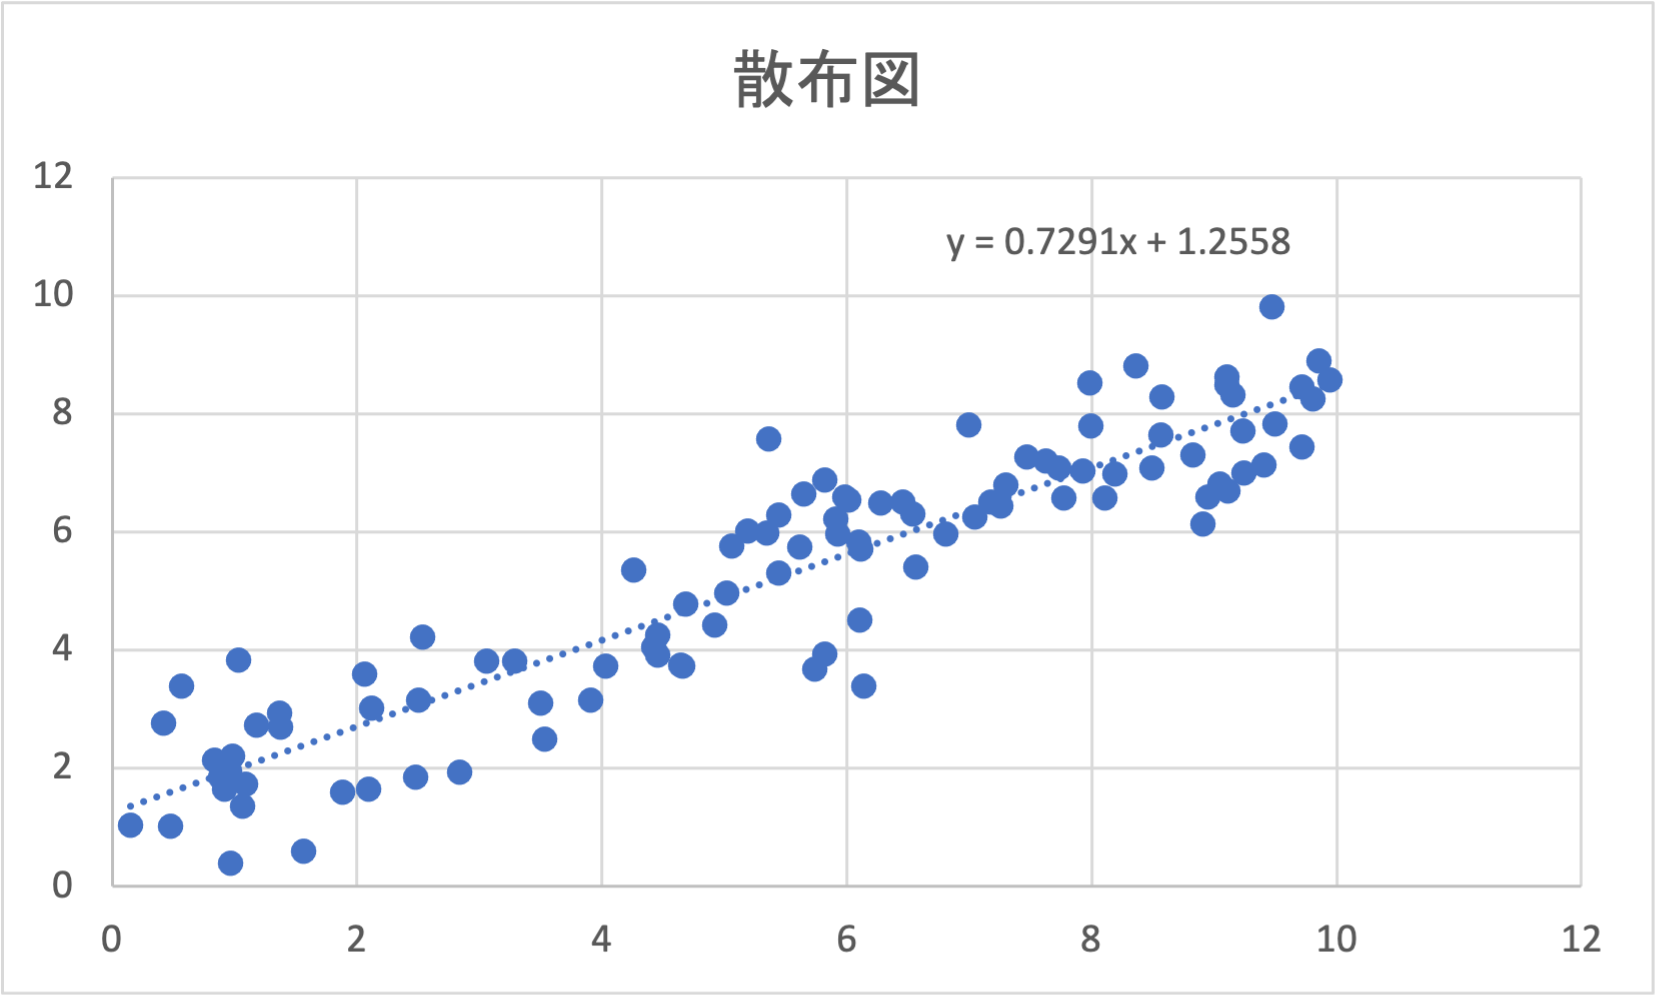
\includegraphics[height=7cm,width=10cm]{sanpuzu.png}
  \caption{data.csvの散布図}
\end{center}
\end{figure}
これらの結果よりプログラムapproximate.cは想定通りの動作をしているといえる.
\section{4.前ページの2〜3を100回繰り返して得られた100個の傾きの値に対して,ヒストグラムを作成せよ.}
generate-data.cとapproximate.cをそれぞれコピーしてmainから100回呼び出せるように変更する.
実際のプログラムをソースコード\ref{main}に示す.行数もそこまで多くないのでそのまま一つのファイルに書き下す.
\begin{lstlisting}[label=main, caption=main.c]
  #include <stdio.h>
  #include <stdlib.h>
  #include <math.h>
  #include <time.h>
  #include <unistd.h>
  #include <string.h>
  
  #define N 10000
  double approximate(const char* filename) {
      int n = 0;
      double x[N],y[N];
      FILE*fp = stdin;
  
      fp = fopen(filename,"r");
      while(fscanf(fp,"%lf,%lf",&x[n],&y[n]) != EOF) {
          n++;
      }
  
      fclose(fp);
      double a,b,s1,s2,avex,avey,temp1=0,temp2=0,sumx=0,sumy=0;
      for (int i = 0; i < n; i++) {
         temp1 += x[i]* y[i];
         temp2 += pow(x[i],2);
         sumx += x[i];
         sumy += y[i];
      }
   
      s1 = (1/(double)(n))*temp1;
      s2 = (1/(double)(n))*temp2;
      avex =(1/(double)(n))* sumx;
      avey =(1/(double)(n))* sumy;
      a = (s1-(avex*avey))/(s2-pow(avex,2));
      b = ((avey*s2)-(avex*s1))/(s2-pow(avex,2));
      printf("傾きa = %g,切片b= %g\n",a,b);
      remove(filename);
      return a;
  }
  
  #define randDouble ((double)rand()+1.0)/((double)RAND_MAX+2.0) // 0以上1未満の実数値の乱数を生成
  
  double rand_normal(double mu, double sigma)
  {
    double e = sqrt(-2.0*log(randDouble)) * sin(2.0*M_PI*randDouble);
    return mu + sigma*e;
  }
  
  int generate_data(const char* filename, int n)
  {
      FILE *file;
      // ファイルを書き込みモードでオープン
      file = fopen(filename, "w");
      
      if (file == NULL){
              printf("ファイルをオープンできませんでした。\n");
              return 1;
      }
  
      int i= 100;
      double a = 0.7, b = 1.2, e;
      double x, y;
  
      srand((unsigned int)time(NULL));
      rand();
      for(i=0; i<n; i++){
          x = randDouble * 10.0;
          e = rand_normal(0,1);
          y = a * x + b + e;
          fprintf(file, "%.3lf,%.3lf\n",x,y);
      }
      fclose(file);
      sleep(1);
      return 0;
  }
  
  int main(int argc, char *argv[])
  {
      FILE *file;
      // ファイルを書き込みモードでオープン
      int datasize = 100;
      char slopefilename[100];
      if(argc >= 2)
      datasize = atoi(argv[1]);
      sprintf(slopefilename,"slope%d.csv",datasize);
      file = fopen(slopefilename, "w");
      
      if (file == NULL){
              printf("ファイルをオープンできませんでした。\n");
              return 1;
      }
      for(int i=0; i<100; i++)
      {
          char filename[100] = "data.csv";
         
          generate_data(filename,100);
          double slope = approximate(filename);
          fprintf(file, "%lf\n",slope);
      }
      fclose(file);
      return 0;
  }  
\end{lstlisting}
この実行結果のslope100.csvを表計算ソフトで読み込みヒストグラムを作成する.
結果は以下の通りとなった.
\begin{figure}[H]
  \begin{center}
  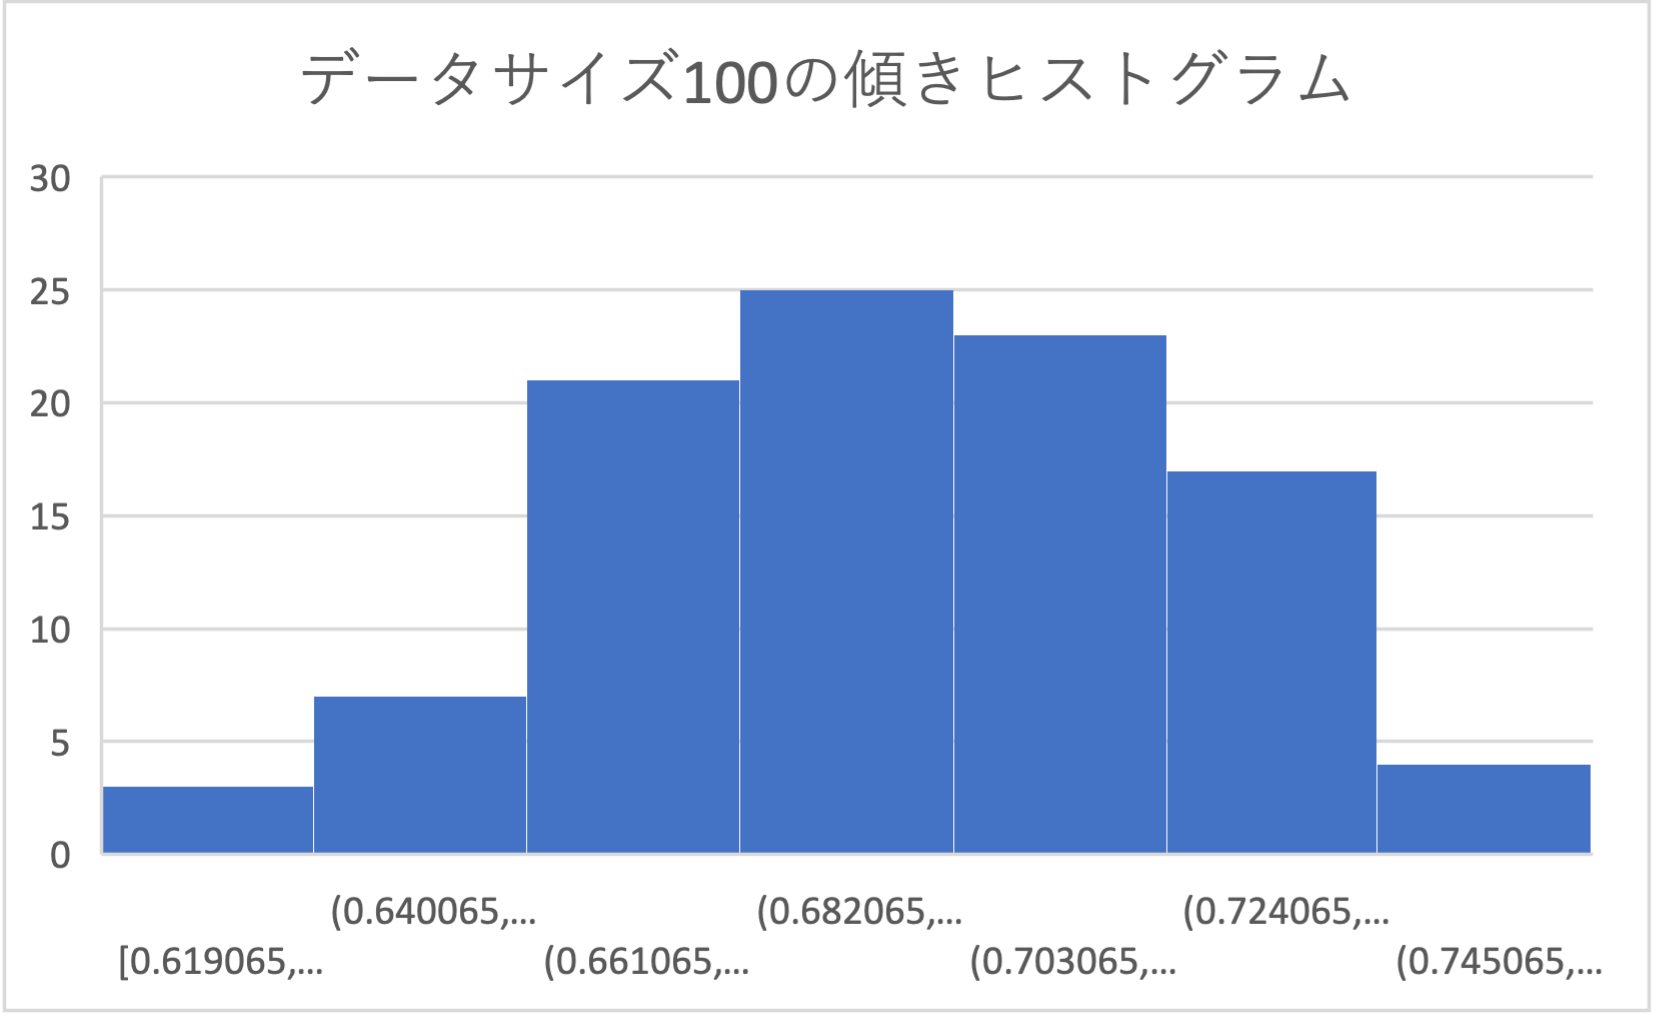
\includegraphics[height=7cm,width=10cm]{2-2-100.png}
  \caption{データサイズ100の傾きのヒストグラム}
\end{center}
\end{figure}
\section{5.前ページの2 で生成されるデータサイズ(=データ対の個数n)を変える(例えば,1000や10000にする)ことで,ヒストグラムがどのようになるかを観察せよ.}
ソースコード\ref{main}に引数1000や10000を与えてデータを取り出す.
4と同様に表計算ソフトで読み込みヒストグラムを作成する.
\begin{figure}[H]
  \begin{center}
  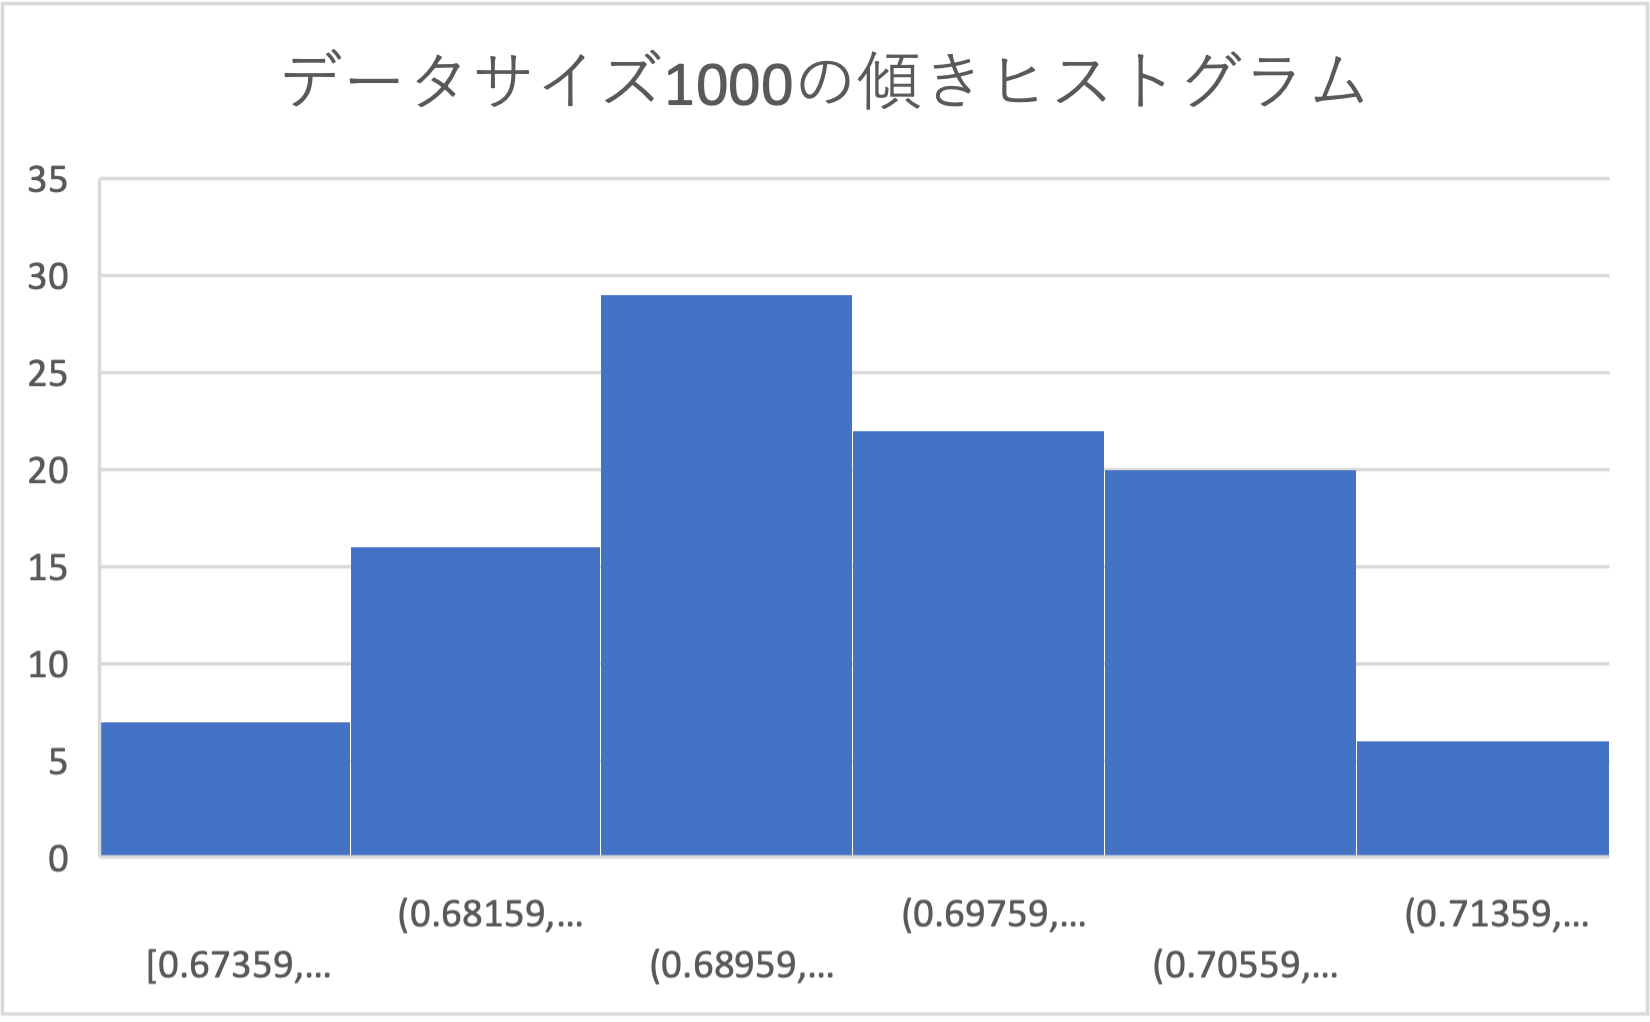
\includegraphics[height=7cm,width=10cm]{2-2-1000.png}
  \caption{データサイズ1000の傾きのヒストグラム}
\end{center}
\end{figure}
\begin{figure}[H]
  \begin{center}
  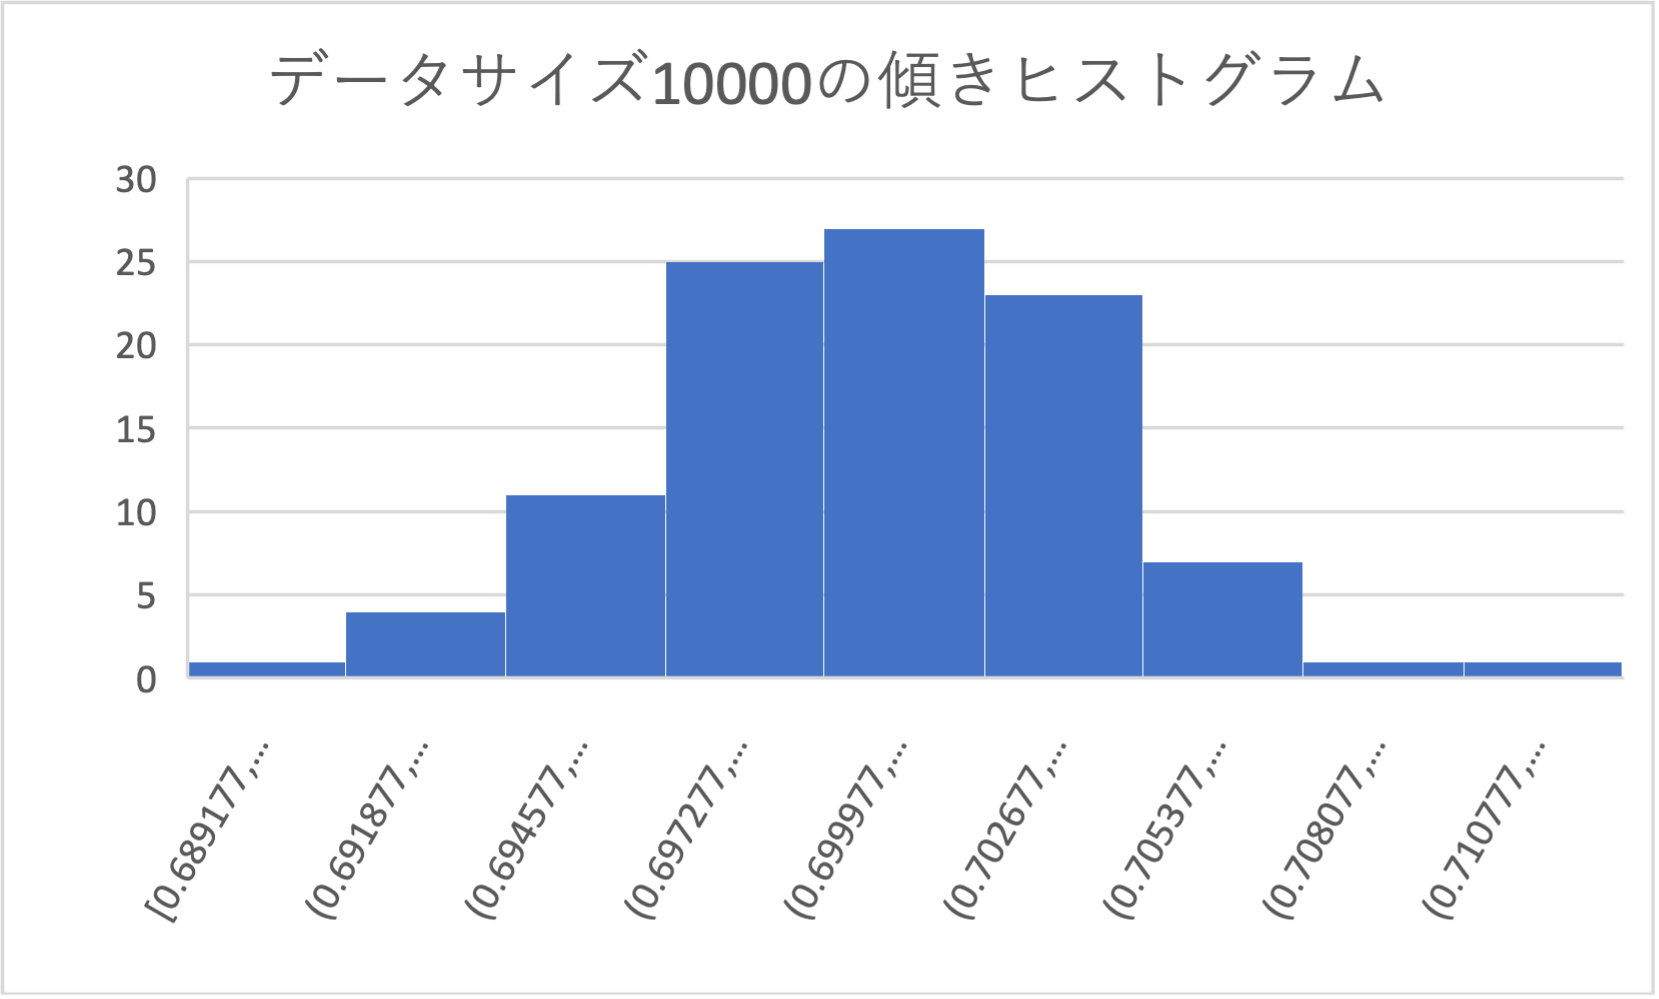
\includegraphics[height=7cm,width=10cm]{2-2-10000.png}
  \caption{データサイズ10000の傾きのヒストグラム}
\end{center}
\end{figure}
\section{6.上記の4〜5を通じて,実験によりわかったことや,その原因を考察して,レポートにまとめよ.}
傾きのヒストグラムをそれぞれ比較してみるとデータサイズが大きくなるに連れて,傾きは0.7から遠い値が少なくなっている.たとえばデータサイズが100のとき一番小さい値が0.619,データサイズが1000のとき一番小さい値が0.673,データサイズが10000のとき一番小さい値が0.689とどんどん0.7に近くなって言っているのがわかる.

このことより,データサイズの数を増やせば増やすほど,0.7に近くなっていくと想定できる.よってデータ数が多いほど最小二乗法の近似式の精度が高くなることがわかる.

実際に自身で数個から数十個程度のデータをとりだしてx軸,y軸のグラフに点をうち,すべての点に近い線を引こうとすると数個の点と数十個の点だと大きくずれが生じる.
ある程度相関のある測定した2つの数,たとえば身長と体重というある程度個人差があるものでもデータの数が多くなれば近似式はより正確になる.
現実にありえる程度に極端に背が高く体重が軽い人が100人のデータの中に混じっていればかなりの誤差が生じるが10000人の中に一人混じっていると極端な数値の人より一般的な数値の人の数のほうが圧倒的に多くなるので
近似式は正確になるだろう.
このように少ないデータに現実にありえる大きく外れた値が混じってしまうと誤差が大きくなってしまうが,データ数が多い場合は大きく外れた値は相対的に少なくなるので誤差も少なくなる.このことがデータサイズの数によって,ヒストグラムが変化する原因だといえる.
\end{document}